\documentclass[10pt]{beamer}

%PTBR
%\usepackage[brazilian]{babel}
\usepackage[utf8]{inputenc}
\usepackage[T1]{fontenc}
\usepackage{bm}
\usepackage{graphicx}
\usepackage[absolute,overlay]{textpos} %pacote para posicionar o logo na primeira página
%\usepackage[dvipsnames]{xcolor}


% Ununbered footnote
\usepackage{blindtext}
\newcommand\blfootnote[1]{%
\begingroup
\renewcommand\thefootnote{}\footnote{#1}%
\addtocounter{footnote}{-1}%
\endgroup
}

\usetheme[progressbar=frametitle]{metropolis}
\usepackage{appendixnumberbeamer}

\usepackage{booktabs}
\usepackage[scale=2]{ccicons}

\usepackage{pgfplots}
\usepgfplotslibrary{dateplot}

\usepackage{xspace}
\newcommand{\themename}{\textbf{\textsc{metropolis}}\xspace}

\usepackage{MacrosSlides}
\usetikzlibrary{arrows.meta} %TIKZ
%\usetikzlibrary{tikzmark} %Arrows over tables (?)
\usetikzlibrary{shapes.misc, positioning}

%\definecolor{teal}{rgb}{0.0, 0.5, 0.5}
%\definecolor{darkorange}{rgb}{1.0, 0.55, 0.0}

\title{Rational defeasible subsumption in DLs with nested quantifiers}
\subtitle{the case of $\mathcal{ELI}_\bot$}

\titlegraphic{%
  \begin{picture}(0,0)
    \put(305,-120){\makebox(0,0)[rt]{\includegraphics[width=6cm]{img/logos.png}}}
  \end{picture}}

\date{August 7th 2022}
\author{\underline{Igor de Camargo e Souza Câmara$^{1}$} \\ Anni-Yasmin Turhan$^{2}$}
\institute{$^{1}$University of São Paulo \\ $^{2}$Dresden University of Technology }


\begin{document}

\begin{frame}[plain]
  \titlepage
\end{frame}

%
% Outline
%

\begin{frame}[fragile] {Outline}

    \Large{
    \begin{itemize}
      \item  Bring defeasible reasoning to DLs.
      \item Several reasoning methods for DDLs suffer from \textbf{quantification neglect}.
      \item \textbf{Typicality models} overcome this for \ELbot.
      \item We extend this approach for inverse roles (\ELIbot).
    \end{itemize}
    }
\end{frame}

%
% Description Logics
%

\begin{frame}[fragile]{Description Logics}
  %\begin{center}

  \Large {
    Concepts
  }

{\large
  $C \grammar \top \mid \bot \mid A \mid C\sqcap D \mid \exists r.C$
}
  \vspace{2mm}
    
    \Large{
      Semantics
    }

    \large{
    $\Imc = (\Delta^{\Imc}, \cdot^{\Imc})$
    }

    { \normalsize
    \begin{table}[ht]
      \begin{tabular}{c r}
      %\cline{1-2}
       $\top^\Imc$ & $\Delta^\Imc$ \\ %\cline{1-2}
       $\bot^\Imc$ & $\emptyset$ \\ %\cline{1-2}
       $(C\sqcap D)^\Imc$ & $C^\Imc\cap D^\Imc$   \\ %\cline{1-2}
       $(\exists r.C)^\Imc$ & $\{x\in\Delta^\Imc \mid \exists y\in\Delta^\Imc\textrm{ s.t. }(x,y)\in r^\Imc\textrm{ and } y\in C^\Imc\}$    \\ %\cline{1-2}
       $(\forall r.C)^\Imc$ & $\{x\in\Delta^\Imc \mid \forall y\in\Delta^\Imc\textrm{ if }(x,y)\in r^\Imc\textrm{, then } y\in C^\Imc\}$  \\ %\cline{1-2}
      \end{tabular}
      \end{table}
    }
  %\end{center}
\end{frame}


%
% Description Logics #2
%

\begin{frame}[fragile]{Description Logics}
  %\begin{center}

    \Large{
      Knowledge Base
    }

    \Large{
      $\Kmc = ({\color{orange}\Tmc}, {\color{teal}\Dmc})$
    }

  %\end{center}

    \vspace{1mm}

\begin{columns}

\begin{column}{.5\textwidth}
    

    \large{\color{orange}$\dlFont{Bird} \sqsubseteq \dlFont{Animal} \sqcap \exists \dlFont{has}.\dlFont{Wings}$
    $\dlFont{Penguin} \sqsubseteq \dlFont{Bird}$}
\end{column}

\begin{column}{.5\textwidth}
    
    \large{ \color{teal} $\dlFont{Bird} \definc \dlFont{Flies}$

    $\dlFont{Bird} \definc \dlFont{Feathered}$

    $\dlFont{Penguin} \sqcap \dlFont{Flies} \definc \bot$}
\end{column}

\end{columns}

\vspace{1mm}

\pause
\Large{Checking subsumption by canonical models}

\large{
$\Imc^{\Kmc} \models C \sqsubseteq D$ iff $C \in D^{\Imc^{\Kmc}}$
}

\pause
%\begin{center}
  \vspace{0.5cm}
  \Large{Checking Defeasible Subsumption}
%\end{center}

\vspace{1mm}
\large{
$\Kmc \models \dlFont{Penguin} \definc \dlFont{Feathered}?$
}



\end{frame}

%
% Materialisation-based reasoning -- Intro & Notation
%

\begin{frame}[fragile]{Materialisation-based reasoning\blfootnote{\textbf{[Casini-Straccia-JELIA'10]}}}
  
  %\begin{center}
    \Large {\textbf{Materialisation}}

    \Large{
  $C \definc D \Rightarrow \lnot C \sqcup D$
    }

    \Large{\textbf{Materialisation-based Reasoning}}
%\end{center}

{\large
$\Kmc \models_{\mathsf{mat}} C \definc D$ \emph{iff } $\Tmc \models C \sqcap \overline{S} \sqsubseteq D \text{, where }S \subseteq \Dmc$
}

\pause
%\begin{center}
  \Large{\textbf{Rational materialisation-based reasoning}}
%\end{center}

{\large
$\Dmc = \Emc_0 \supset \Emc_1 \supset \dots \supset \Emc_n = \emptyset$
}
\end{frame}

%
% Rational Reasoning -- Example 1 [1/]
%

\begin{frame}{Example}
  \begin{tikzpicture}

    % 
    \draw[teal,thick,fill=teal!30,rounded corners] (-0.2, 3) rectangle (4.2,6); %TBox
        \node[] at (2, 6.4) (TBox) {{\Large \color{teal} $\Tmc$}};

    \draw[purple,thick,fill=purple!30,rounded corners] (5, 3) rectangle (9,6); %DBox E_0
        \node[] at (7, 6.4) (DBox) {{\Large \color{purple} $\Dmc = \Emc_0$}};

    \draw[orange,thick,fill=orange!30,rounded corners] (5.2, 4.7) rectangle (8.8,5.8); %TBox
        \node[] at (9.4, 5.2) (DBox) {{\Large \color{orange} $\Emc_1$}};

    % T - Axioms
    \node [] at (2, 5.6) (TAxiom0) {\large $\dlFont{Cat} \sqsubseteq \exists \dlFont{eats}.\dlFont{Bird}$};
    \node [] at (2, 5) (TAxiom1) {\large $\dlFont{Penguin} \sqsubseteq \dlFont{Bird}$}; 
    \node [] at (2, 4.4) (TAxiom2) {\large $\dlFont{Sparrow} \sqsubseteq \dlFont{Bird}$};
    \node [] at (2, 3.8) (TAxiom3) {\large $\dlFont{King Penguin} \sqsubseteq \dlFont{Penguin}$};
    
    % E_0 - Axioms
    \node [] at (7, 5.2) (E_0Axiom1) {\large $\dlFont{Penguin} \definc \lnot \dlFont{Flies}$};

    % E_1 - Axioms
    \node [] at (7, 4.3) (E_1Axiom1) {\large{$\dlFont{Bird} \definc \dlFont{Flies}$}};
    \node [] at (7, 3.5) (E_1Axiom2) {\large{$ \dlFont{Bird} \definc \dlFont{Feathered}$}};

    %\node [] at (5, 1.5) (Entailment) {\large $\Kmc  \matModels{\mathsf{rat}} \dlFont{King Penguin} \definc \lnot \dlFont{Flies}$?};

%\pause

%\node [] at (5, 0.5) (Entailment) {\large $\Tmc \models \dlFont{King Penguin} \sqcap {\color{orange} \overline{\Emc_1}} \sqsubseteq \lnot \dlFont{Flies}$};

    \end{tikzpicture}
\end{frame}

%
% Quantification Neglect [1]
%
%\begin{frame}{Example 2 -- Quantification Neglect}
%    \begin{tikzpicture}
%  
      % 
%      \draw[gray,thick,fill=gray!30,rounded corners] (-0.2, 3) rectangle (4.2,6); %TBox
%          \node[] at (2, 6.4) (TBox) {{\Large \color{orange} $\Tmc$}};
  
 %     \draw[orange,thick,fill=orange!30,rounded corners] (5, 3) rectangle (9,6); %DBox E_0
 %         \node[] at (7, 6.4) (DBox) {{\Large \color{gray} $\color{orange} \Emc_0$}};
  
 %     \draw[orange!30,thick,fill=orange!30,rounded corners] (5.2, 4.7) rectangle (8.8,5.8); %TBox
 %         \node[] at (9.4, 5.2) (DBox) {{\Large $\Emc_1$}};
  
      % T - Axioms

    % T - Axioms
%    \node [] at (2, 5.6) (TAxiom0) {\large $\dlFont{Cat} \sqsubseteq \exists \dlFont{eats}.\dlFont{Bird}$};
%    \node [] at (2, 5) (TAxiom1) {\large $\dlFont{Penguin} \sqsubseteq \dlFont{Bird}$}; 
%    \node [] at (2, 4.4) (TAxiom2) {\large $\dlFont{Sparrow} \sqsubseteq \dlFont{Bird}$};
%    \node [] at (2, 3.8) (TAxiom3) {\large $\dlFont{King Penguin} \sqsubseteq \dlFont{Penguin}$};
      
      % E_0 - Axioms
%      \node [] at (7, 5.2) (E_0Axiom1) {\large $\dlFont{Penguin} \definc \lnot \dlFont{Flies}$};
  
      % E_1 - Axioms
%      \node [] at (7, 4.3) (E_1Axiom1) {\large{$\dlFont{Bird} \definc \dlFont{Flies}$}};
%      \node [] at (7, 3.5) (E_1Axiom2) {\large{$ \dlFont{Bird} \definc \dlFont{Feathered}$}};

    % ENTAILMENT
%    \node [] at (5, 1.5) (Entailment) {\large $\Tmc \Large{\not\models} \dlFont{Cat} \sqcap {\color{orange} \overline{\Emc_0}} \sqsubseteq \exists \dlFont{eats}.\dlFont{Flies}$};

%      \end{tikzpicture}
%  \end{frame}

%%%%%%%%%%%%%%%%%%%%%%%%%%%%%%%%%%%%%%%%%%%%%%%%%
% Section 2: Introduction to Typicality Models  %
%%%%%%%%%%%%%%%%%%%%%%%%%%%%%%%%%%%%%%%%%%%%%%%%%

%\section{Typicality Models}

\begin{frame}[fragile]{Typicality Models for \ELbot\blfootnote{[Pensel-Turhan-IJAR'18]}}

  %\begin{center}
\Large{
  \textbf{Typicality Domains}} 
  
\large{
  $\typel{C}{\Umc}$ represents $C \sqcap \overline{\Umc}$
  
  $\Umc \subseteq \Dmc$
  } 

\pause
\vspace{0.5cm}
\Large{
  \textbf{Satisfaction}} 
    
  \large{
    $\Imc \models C \definc D$ 
    
    iff
    
    $\typel{C}{\Emc_i} \in D^{\Imc}$ for every maximal $\Emc_i$ \wrt $C$ in the domain.
    } 
%\end{center}
\end{frame}


%
% Minimal Rational Domain 
%

\begin{frame}[fragile]{Minimal Rational Typicality Model for \ELbot}

\vspace{0.3cm}
\begin{figure}
  \centering
      \includegraphics[width=\textwidth]{img/verboseratmod.png}
  \end{figure}

\end{frame}

%
% Upgrading Edges
%

%\begin{frame}{Upgrading Edges From the Minimal Typicality Model for \ELbot}
%  \begin{center}
%    { \Large 
%      \vspace{0.3cm}
%      $\Imc \models \dlFont{Cat} \definc \exists \dlFont{eats}.\dlFont{Flies}$
%    }
%  \end{center}

%  \vspace{0.3cm}
%\begin{figure}
%  \centering
%      \includegraphics[width=\textwidth]{img/verboseratmod2.png}
%  \end{figure}
%\end{frame}

%%%%%%%%%%%%%%%%%%%%%%%%%%%%%%%%%%%%%%%%%%%
% Section 3: ELI_Bot & Typicality Models  %
%%%%%%%%%%%%%%%%%%%%%%%%%%%%%%%%%%%%%%%%%%%

%\section{Introducing Inverse Roles}

%
% Overview
%

\begin{frame}{Lifting defeasible entailment to inverse roles -- How to extend typicality models?}
 
 \Large{
(1.) {\color{orange}Adjusting the domain;}

(2.) Identifying edge owners;
 
(3.) Recovering the model property.
}

\end{frame}


%
% Domain
%

\begin{frame}{Adjusting the Domain}
  \begin{center}
    {\color{purple}
    \Large{\ELbot}

      \large{
        $C \sqsubseteq \exists r.D \Rightarrow (C,D) \in r^{\minrattypp}$
    }}
  \end{center}
{\large $A \sqsubseteq \exists r.B, A \sqsubseteq \forall r.C$}

  \centering{
  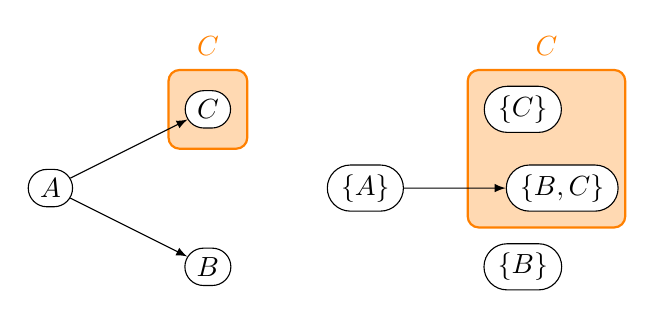
\begin{tikzpicture}
    \draw[orange,thick,fill=orange!30,rounded corners] (1.5, 1.5) rectangle (2.5,2.5); %C Concept
      \node[] at (2,2.8) (CCon) {{\color{orange}$C$}};

    \node[rounded rectangle, fill=white, draw] at (0,1) (A) {$A$};
    \node[rounded rectangle, fill=white, draw] at (2,0) (B) {$B$};
    \node[rounded rectangle, fill=white, draw] at (2,2) (C) {$C$};

    \draw[-latex](A) to (B);
    \draw[-latex](A) to (C);

    \pause

    \draw[orange,thick,fill=orange!30,rounded corners] (5.3, 0.5) rectangle (7.3,2.5);
      \node[] at (6.3,2.8) (CCon) {{\color{orange}$C$}};

    \node[rounded rectangle, fill=white, draw] at (4,1) (A2) {$\{A\}$};
    \node[rounded rectangle, fill=white, draw] at (6,0) (B2) {$\{B\}$};
    \node[rounded rectangle, fill=white, draw] at (6,2) (C2) {$\{C\}$};
    \node[rounded rectangle, fill=white, draw] at (6.5,1) (BC) {$\{B,C\}$};

    \draw[-latex](A2) to (BC);

    %\node[] at (3.5, -1) (text) {\large $C \sqsubseteq \exists r.M$ \textbf{ and } $M$ \text{ is maximal } \wrt $\Kmc, C, r \Rightarrow (C,M) \in r^{\minrattypp}$ };
  \end{tikzpicture}}

\end{frame}

%
% Overview 2
%

\begin{frame}{Overview}
  \Large{
 (1.) Adjusting the domain;
 
 (2.) {\color{orange} Identifying edge owners;}
  
 (3.) Recovering the model property.
 }
 \end{frame}

%
% Causal Direction of the Edges
%

\begin{frame}{Causal Direction of the Edges}

  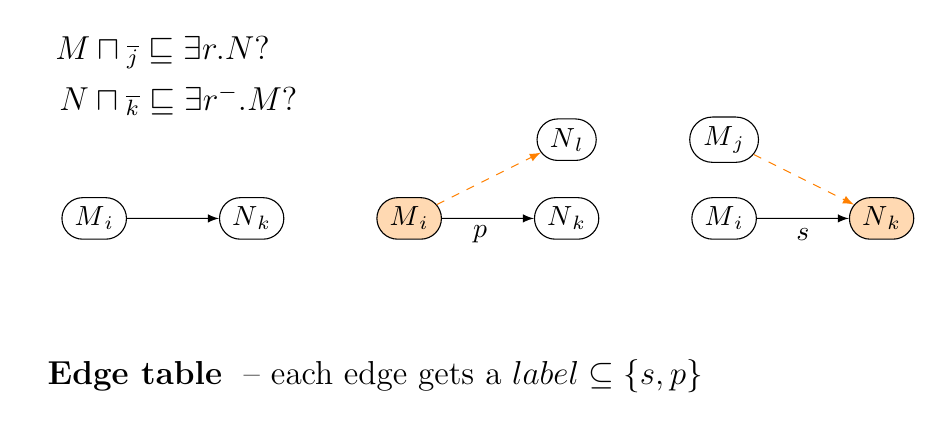
\begin{tikzpicture}

    \node[rounded rectangle, fill=white, draw] at (0,0) (Mi) {$\typel{M}{\Emc_i}$};

    \node[] at (0.8,2.1) (N) {\large{ $M \sqcap \overline{\Emc_j} \sqsubseteq \exists r.N?$}};
    \node[] at (1,1.5) (N) {\large{ $N \sqcap \overline{\Emc_k} \sqsubseteq \exists r^{-}.M?$}};
    \node[rounded rectangle, fill=white, draw] at (2,0) (Nk) {$\typel{N}{\Emc_k}$};
    \draw[-latex](Mi) to (Nk);

    %%% 2 %%%
      \pause

    \node[rounded rectangle, fill=orange!30, draw] at (4,0) (Mi2) {$\typel{M}{\Emc_i}$};

    \node[rounded rectangle, fill=white, draw] at (6,0) (Nk2) {$\typel{N}{\Emc_k}$};
    \node[rounded rectangle, fill=white, draw] at (6,1) (Nl2) {$\typel{N}{\Emc_l}$};

    \draw[-latex](Mi2) to (Nk2);
    \draw[-latex, dashed, orange](Mi2) to (Nl2);
      \node[] at (4.9,-0.2) (pred) {$p$};

    %%% 3 %%%

    \node[rounded rectangle, fill=white, draw] at (8,0) (Mi3) {$\typel{M}{\Emc_i}$};
    \node[rounded rectangle, fill=white, draw] at (8,1) (Mj) {$\typel{M}{\Emc_j}$};

    \node[rounded rectangle, fill=orange!30, draw] at (10,0) (Nk3) {$\typel{N}{\Emc_k}$};

    \draw[-latex](Mi3) to (Nk3);
    \draw[-latex, dashed, orange](Mj) to (Nk3);
      \node[] at (9,-0.2) (suc) {$s$};

      \node[] at (3.5,-2) (N) {\large{ \textbf{Edge table} \text{ -- each edge gets a $label \subseteq \{s, p\}$}}};

  \end{tikzpicture}

%\vspace{5mm}
%\begin{center}{\Large
%  \textbf{Edge table} -- each edge gets a $label \subseteq \{s, p\}$.}
%\end{center}

\end{frame}


% Selecting Candidates + Edge Table ?

%
% Overview 3
%

\begin{frame}{Overview}
  \Large{
 (1.) Adjusting the domain;
 
 (2.) Identifying edge owners;
  
 (3.) {\color{orange} Recovering the model property}.
 }
 \end{frame}

 %
 % Recovering in ELBot + the problem
 %

 \begin{frame}{Fixing violations of GCIs in \ELIbot TBoxes}

  \begin{center}
  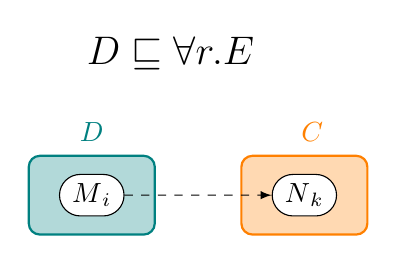
\begin{tikzpicture}

  \draw[teal,thick,fill=teal!30,rounded corners] (0.2, -0.5) rectangle (1.8,0.5); %D Concept
    \node[] at (1,0.8) (DCon) {{\color{teal}$D$}};

  \draw[orange,thick,fill=orange!30,rounded corners] (2.9, -0.5) rectangle (4.5,0.5); %C Concept
    \node[] at (3.8,0.8) (CCon) {{\color{orange}$C$}};

    \node[rounded rectangle, fill=white, draw] at (1,0) (Mi) {$\typel{M}{\Emc_i}$};
    \node[rounded rectangle, fill=white, draw] at (3.7,0) (Nk) {$\typel{N}{\Emc_k}$};

    %\node[] at (2,2.5) (N) {\Large{$\exists r.C \sqsubseteq D$}};
    \node[] at (2,1.8) (N) {\Large{$D \sqsubseteq \forall r.E$}};

    \draw[-latex, dashed](Mi) to (Nk);

  \end{tikzpicture}
\end{center}
\end{frame}



\begin{frame}[fragile] {Two kinds of repair}

  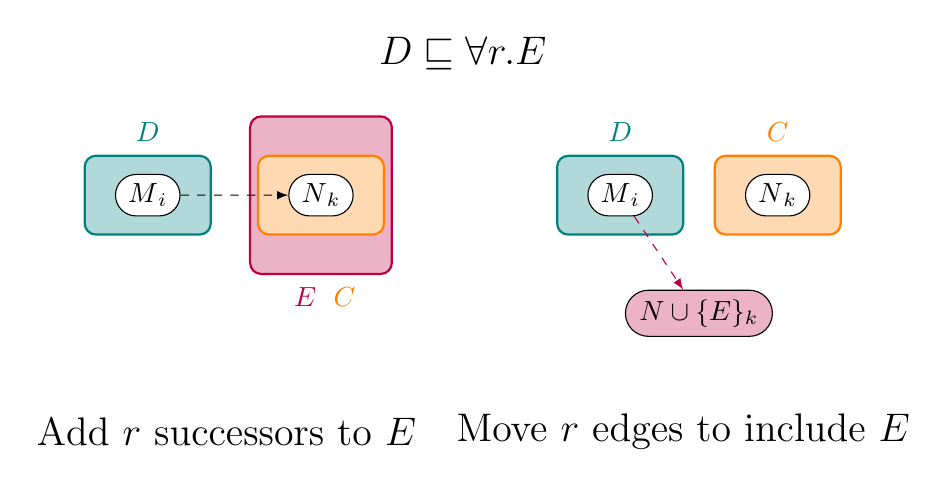
\begin{tikzpicture}
    
  \node[] at (5,1.8) (N) {\Large{$D \sqsubseteq \forall r.E$}};

  \draw[teal,thick,fill=teal!30,rounded corners] (0.2, -0.5) rectangle (1.8,0.5); %D Concept
    \node[] at (1,0.8) (DCon) {{\color{teal}$D$}};
  \node[rounded rectangle, fill=white, draw] at (1,0) (Mi) {$\typel{M}{\Emc_i}$};

  % Fix #2
  \node[] at (2,-3) (N) {{\Large\text{Add $r$ successors to $E$}}};

  \draw[purple,thick,fill=purple!30,rounded corners] (2.3, -1) rectangle (4.1,1); %E Concept
    \node[] at (3.5,-1.3) (CCon2) {{\color{orange}$C$}};
    \node[] at (3,-1.3) (CCon2) {{\color{purple}$E$}};

  \draw[orange,thick,fill=orange!30,rounded corners] (2.4, -0.5) rectangle (4,0.5); %C Concept

  \node[rounded rectangle, fill=white, draw] at (3.2,0) (Nk) {$\typel{N}{\Emc_k}$};
  \draw[-latex, dashed](Mi) to (Nk);
  
  %%%%%%%%%%%%%%%% 3 %%%%%%%%%%%%%%%%%

  \draw[teal,thick,fill=teal!30,rounded corners] (6.2, -0.5) rectangle (7.8,0.5); %D Concept
    \node[] at (7,0.8) (DCon3) {{\color{teal}$D$}};

  \draw[orange,thick,fill=orange!30,rounded corners] (8.2, -0.5) rectangle (9.8,0.5); %C Concept
    \node[] at (9,0.8) (CCon3) {{\color{orange}$C$}};

    
    \node[rounded rectangle, fill=white, draw] at (7,0) (Mi2) {$\typel{M}{\Emc_i}$};
    \node[rounded rectangle, fill=white, draw] at (9,0) (Nk2) {$\typel{N}{\Emc_k}$};
    \node[rounded rectangle, fill=purple!30, draw] at (8,-1.5) (Nk2) {$\typel{N \cup \{E\}}{\Emc_k}$};

    \draw[-latex, dashed, purple](Mi2) to (Nk2);

  % Fix #3
  \node[] at (7.8,-3) (N) {\Large{\text{Move $r$ edges to include $E$}}};

  \end{tikzpicture}
\end{frame}

 %
 % Edge Dependency and the solution
 %


%%%%%%%%%%%%%%%%%% NESTED REASONING %%%%%%%%%%%%%%%%%%%%%%%%%%

%\section{Nested Reasoning}

%
% Nested reasoning
%

\begin{frame}[fragile] {Nested Reasoning}

\begin{center}
  \Large{
    Skeptical Reasoning 

    \large $\Kmc \ratModelsnest A \definc B$ \textit{ iff }$\typel{\{A\}}{\Emc_{\min}} \in B^{\Imc}$
  }
\end{center}

\pause

  \begin{columns}

    \begin{column}{.5\textwidth}
{\Large 
\begin{align*}
  \Tmc = \{ & \dlFont{Penguin} \sqsubseteq \dlFont{Bird}, \\ 
  & \dlFont{Cat} \sqsubseteq \exists \dlFont{eats}.\dlFont{Bird} \} \\ 
  \Dmc = \{ & \dlFont{Penguin} \definc \lnot \dlFont{Flies} \\ 
  & \dlFont{Bird} \definc \dlFont{Flies} \\ 
  & \dlFont{Bird} \definc \dlFont{Feathered} \} 
\end{align*}
}

\end{column}

\begin{column}{.5\textwidth}

  \begin{tikzpicture}
      \draw[teal,thick,fill=teal!30,rounded corners] (0.9, -1.5) rectangle (3.1,-0.5); %Flies Concept
      \node[] at (2,-2) (ECon) {{\color{teal}$\dlFont{Flies}$}};

      \node[rounded rectangle, fill=white, draw] at (0,0) (Catd) {$\typel{\{\dlFont{Cat}\}}{\Emc_0}$};
      \node[rounded rectangle, fill=white, draw] at (2,1) (Bird0) {$\typel{\dlFont{Bird}}{\emptyset}$};
      \node[rounded rectangle, fill=white, draw] at (2,-1) (Birdd) {$\typel{\{\dlFont{Bird}\}}{\Dmc}$};

      \draw[-latex] (Catd) to (Bird0);
      \draw[-latex, dashed] (Catd) to (Birdd);

      \node[] at (2,-3) (Catelflies) {{\color{teal}$\{\typel{\dlFont{Cat}}{\Emc_0}\} \in \exists \dlFont{eats}.\dlFont{Flies}^{\Imc}$ }};
      \node[] at (2,-3.5) (CatDCI) {\color{teal}$\Kmc \ratModelsnest \dlFont{Cat} \definc \exists \dlFont{eats}. \dlFont{Flies}$};

  \end{tikzpicture}
\end{column}

\end{columns}
\end{frame}

%
% Conclusions
%

\begin{frame}[fragile] {Conclusions}

\large{
Summary

\begin{itemize}
  \item Devised semantics for defeasible reasoning in the presence of inverse roles;
  \item Extended reasoning method by typicality models;
  \item Alleviated quantification neglect for \ELIbot under rational closure.
\end{itemize}

Next steps

\begin{itemize}
  \item Alleviate inheritance blocking with relevant closure;
  \item Move to more expressive DLs (Horn DLs);
  \item Treat defeasible reasoning \wrt ABox.
\end{itemize}
}
\end{frame}

%\begin{frame}[fragile] {Conclusions}
%\large{
%\begin{itemize}
%  \item Adapted core ideas from \ELbot TM semantics to \ELIbot for rational reasoning
%    \begin{itemize} \large{
%      \item Introduced a new form of typicality domain;
%      \item Proposed a formal apparatus to deal with the bidirectionality of the edges; 
%      \item Formulated a new upgrade procedure that fixed violations from inverse roles in a meaningful way
%      \item Defined a new direct construction for a maximal typicality model.}
%    \end{itemize}
%  \item Dealt with quantification neglect in rational reasoning the DDL \ELIbot.
%    \end{itemize}
%}
%\end{frame}

%\begin{frame}[fragile] {Future Work}

%{\Large
%\begin{itemize}
%  \item Work with stronger materialisation-based reasoning coverages (e.g. lexicographic, relevant);
%  \item Study complexity of this reasoning procedure;
%  \item Investigate the broader class of horn-DLs;
%  \item Compare with other existing frameworks.
  %\item Work on a set of KLM-like postulates that better capture quantification.
%\end{itemize}
%}
%\end{frame}


%
% Bib
%

%\begin{frame}[allowframebreaks]
%  \frametitle{References}
%  \bibliographystyle{amsalpha}
%  \bibliography{../../biblio.bib}
%\end{frame}

\end{document}




